\section{Fifth Member}
This is the section dedicated to one of the team members, and it should be written individually . It can include a range of things; first subsection is a space for you to point out the strengths and weaknesses of the module, including complaints about the module coordinator Max Wilson. The second section should have a selfie image with Max! The last part of it is the most important one. You will need to write a paragraph about what you have learned in this module. You can write it in \textbf{Bold} if you want or you can use other fonts. 

Please do not forget:
\begin{itemize}
	\item First paragraph should have your comments about the module
	\item Second one, a selfie img with Max
	\item Last one, what you learned in this module.
\end{itemize}

\subsection{Comments about the module}
What I love about this module is the instruction that has given to us are very clear and I did able to understand the steps easily without a lot of questions. Besides, I enjoy the guest lecture too as that is a fantastic experience to me because I can have the chance to learn and listen from the others. However, the only things that I do not like about is that during the lab section some computers were not working for different reasons and this force me to use my own laptop, but I sincerely want to use the lab machine because I believe it is slightly more convenient.

\subsection{Selfie with Max}

\begin{figure}[h]
\caption{Selfie with Max}
\centering
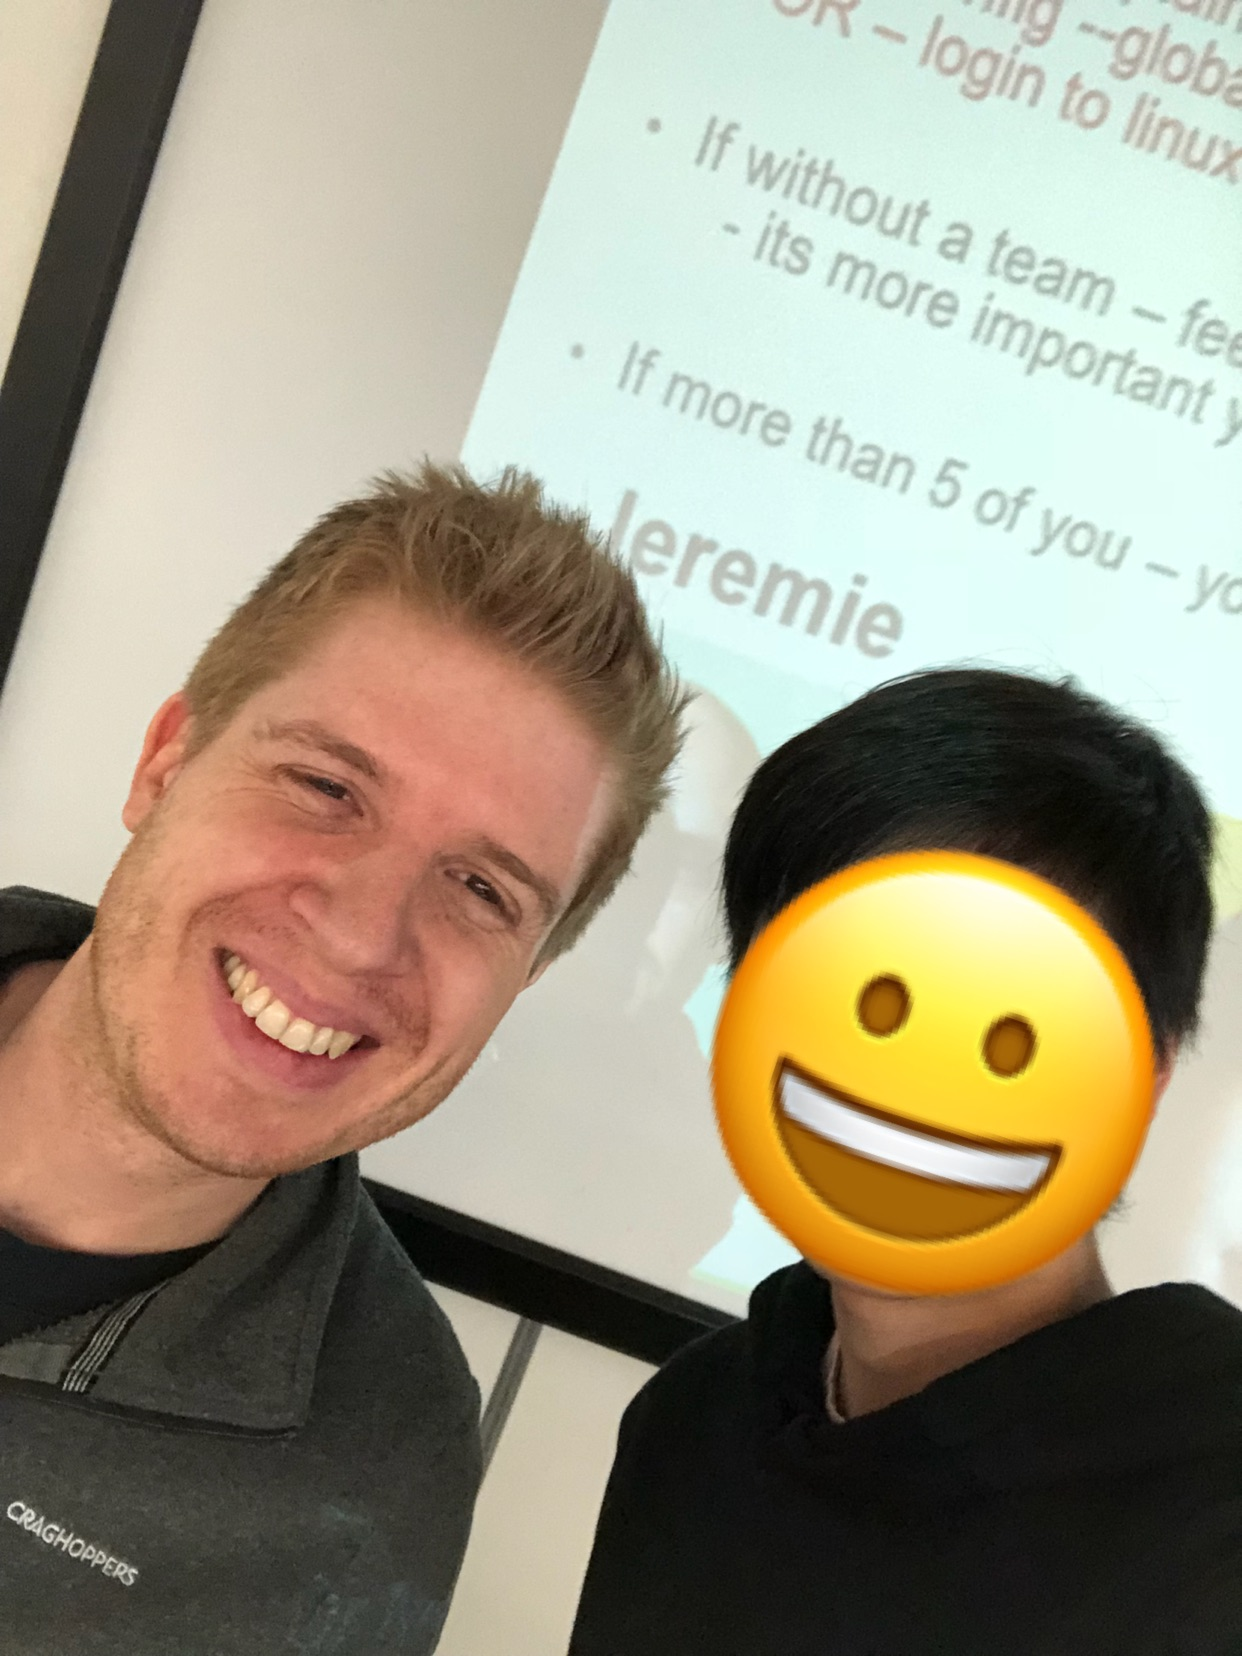
\includegraphics[width=0.5\textwidth]{Smileyface.jpg}
\label{fig:selfie}
\end{figure}

%You can then use the label of the figure to reference it later with the command ${\backslash}ref$. you can comment out the next line to see an example of how it works.

% My selfie with Max is in  Figure~\ref{fig:selfie}.

\subsection{What I have learned in this module}
What I have learnt from this module is that the skills to work with other people and how to work equally. Moreover, I have learnt the most important things which is listen and discuss with my group mates. I believe this is extremely important because if we work as a group we will be able to work much more efficiently and quicker.

